\documentclass{beamer}
\usepackage[utf8]{inputenc}

\usetheme{Madrid}
\usecolortheme{default}
\usepackage{color}
\usepackage{colortbl}

\usepackage{algorithmic}

\def\HiLi{\leavevmode\rlap{\hbox to \hsize{\color{yellow!50}\leaders\hrule height .8\baselineskip depth .5ex\hfill}}}

\begin{document}

\title{Algoritmo Q-Learning} 
\author{Fabrício Barth}
\institute{Insper Instituto de Ensino e Pesquisa}
\date{Fevereiro de 2025}

\maketitle

\begin{frame}{Política de Controle}
	\begin{itemize}
		\item A política de controle desejada é aquela que \textbf{maximiza} os reforços 
		(\textit{reward}) acumulados ao longo do tempo pelo 
		agente.
		\item Em tese, é a política que faz o agente percorrer o \textbf{melhor caminho}. 
	\end{itemize}
	
	%\hspace{1cm}
	
	\begin{center}
		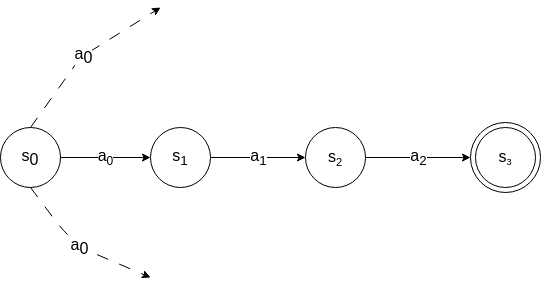
\includegraphics[width=.8\textwidth]{figuras/grafo_rewards_0.png}
	\end{center}
	
\end{frame}


\begin{frame}{Reward acumulado (1/4)}
	
	\begin{center}
		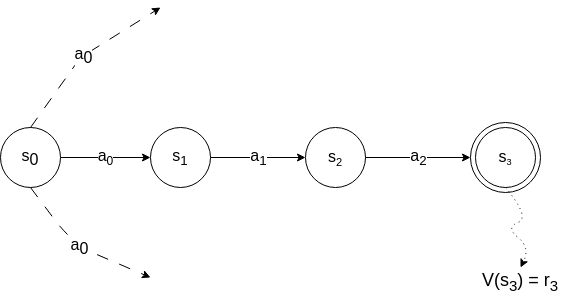
\includegraphics[width=.8\textwidth]{figuras/grafo_rewards_1.png}
	\end{center}
	
	\begin{itemize}	
		\item O valor de um estado final leva-se em consideração apenas o 
		reforço: $V(s_{n}) = r_{n}$.
	\end{itemize}
	
\end{frame}


\begin{frame}{Reward acumulado (2/4)}
	
	\begin{center}
		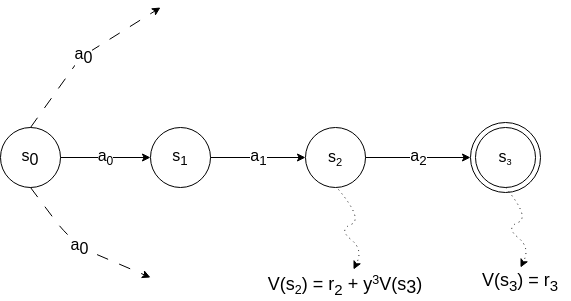
\includegraphics[width=.8\textwidth]{figuras/grafo_rewards_2.png}
	\end{center}
	
	\begin{itemize}	
		\item O $V(s_{2})$ será a soma de $r_{2}$ com o $V(s_{3})$. 
		\item Considerando o fator de desconto $\gamma$, temos: $V(s_{2}) = r_{2} + \gamma^{3} V(s_{3}) $.
		\item O fator de desconto: $0 \leq \gamma < 1$ 
	\end{itemize}
	
\end{frame}

\begin{frame}{Reward acumulado (3/4)}
	
	\begin{center}
		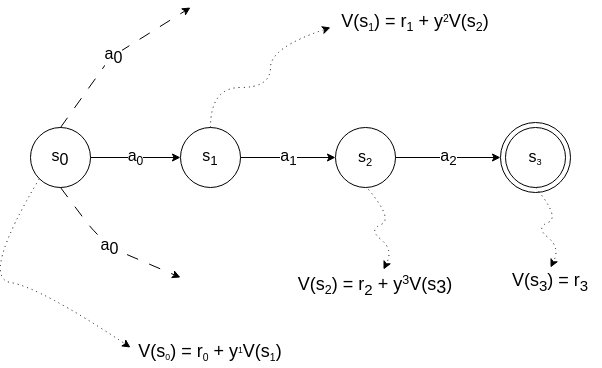
\includegraphics[width=.9\textwidth]{figuras/grafo_rewards_3.png}
	\end{center}
	
\end{frame}

\begin{frame}{Reward acumulado (4/4)}
	
	Desta forma, temos: 
	
	\begin{eqnarray}
		V(s_{0}) = r_{0} + \gamma V(s_{1}) \nonumber \\
		V(s_{0}) = r_{0} + \gamma r_{1} + \gamma^{2} V(s_{2}) \nonumber \\
		V(s_{0}) = r_{0} + \gamma r_{1} + \gamma^{2} r_{2} + \gamma^{3} V(s_{3}) \nonumber \\
		V(s_{0}) = r_{0} + \gamma r_{1} + \gamma^{2} r_{2} + \gamma^{3} r_{3} \nonumber
	\end{eqnarray}
	
	Ou melhor: 
	
	\begin{equation}
		V(s_{0}) = r_{0} + \gamma r_{1} + \gamma^{2} r_{2} + \gamma^{3} r_{3} \cdots + \gamma^{n}r_{n} \nonumber
	\end{equation}
	
	
\end{frame}


\begin{frame}{Fator de desconto $\gamma$}
	
	\begin{itemize}
		%\item Para tarefas episódicas, o retorno é fácil de ser calculado, 
		%pois será a soma de todas as recompensas obtidas pelo agente. 
		%Mas para tarefas contínuas, como a atividade não tem fim e não podemos 
		%somar até o infinito, há a necessidade da inserção de um fator de 
		%desconto ($\gamma$).
		\item O fator de desconto ($\gamma$) é um hiperparâmetro que consiste 
		em um número entre 0 e 1 que define a importância das recompensas futuras 
		em relação a atual	($0 \leq \gamma < 1$).
		\item Valores mais próximos ao 0 dão mais importância a recompensas 
		imediatas enquanto os mais próximos de 1 tentarão manter a importância 
		de recompensas futuras.
	\end{itemize}
\end{frame}


\begin{frame}{Algoritmo Q-Learning}
	
	\begin{itemize}
		\item O algoritmo Q-Learning é um algoritmo do tipo \textit{value-based} que estimam a expectativa de retorno de uma ação $a$ sendo executada em um estado $s$ de acordo com uma política $\pi$: $Q^{\pi}(s,a)$.
		
		\item Para que agente possa identificar uma política de controle ótima este agente 
		precisa criar um \textbf{mapeamento} entre \textbf{estados} ($S$) e \textbf{ações} ($A$).
		
		\item Desta forma o agente consegue identificar qual é a ação $a$ com maior retorno em um determinado estado $s$. 
	\end{itemize}

\end{frame}

\begin{frame}{Algoritmo Q-Learning}
	
\begin{itemize}
	
	\item Este mapeamento é representado por uma função $Q(S,A)$ onde $S$ são 
	todos os estados possíveis ($s_{1}, s_{2}, \cdots$) e onde $A$ são todas as 
	ações possíveis ($a_{1}, a_{2}, \cdots$)

\end{itemize}

	\begin{center}
	\begin{tabular}{ |c|c|c|c|c| } 
		\hline
		 \textbf{Q-table}  & $a_{1}$ & $a_{2}$ & $a_{3}$& $a_{4}$ \\
		 \hline
		$s_{1}$&  &  &  & \\ 
		\hline
		$s_{2}$&  &  &  & \\ 
\hline
		$\cdots$&  &  &  & \\ 
\hline
		$s_{n}$&  &  &  & \\ 
\hline
	\end{tabular}
\end{center}

\end{frame}

\begin{frame}{Algoritmo Q-Learning}

	\begin{block}{}
		Como é que o agente pode saber quais são as melhores ações em cada estado?
	\end{block}

\pause

	\begin{itemize}
		\item A ideia é fazer com que o agente aprenda a função de mapeamento $Q(S,A)$. 
		Ou seja, que seja capaz de identificar qual é a melhor ação para cada estado 
		através das suas \textbf{experiências}. 
		\item \textit{Testando} \textbf{infinitas} vezes o ambiente. 
		Ou seja, \textit{testando} \textbf{muitas} vezes as combinações entre 
		\textbf{estados} ($S$) e \textbf{ações} ($A$). 
	\end{itemize}

\end{frame}

\begin{frame}{Algoritmo Q-Learning} 
	\begin{algorithmic} 
		\STATE \emph{\textbf{function} Q-Learning(env, $\gamma$, $\alpha$, episódios)}
		\STATE inicializar os valores de $Q(s, a)$ arbitrariamente
		\FOR {todos os episódios}
		\STATE inicializar $s$ a partir de $env$
		\REPEAT
		\STATE escolher uma ação $a$ para um estado $s$
		\STATE executar a ação $a$
		\STATE observar a recompensa $r$ e o novo estado $s'$ 
		\STATE \HiLi $Q(s,a) \leftarrow$ atualizando a partir das experiências 
		\STATE$s  \leftarrow s'$
		\UNTIL {$s$ ser um estado final}
		\ENDFOR
		\STATE \textbf{return} $Q(s, a)$
	\end{algorithmic}

\vspace{0.2cm}
\small
Poderíamos simplesmente: $Q(s,a) \leftarrow r$. Será que funciona? 

\end{frame}


\begin{frame}{Algoritmo Q-Learning} 
	\begin{algorithmic} 
		\STATE \emph{\textbf{function} Q-Learning(env, $\gamma$, $\alpha$, episódios)}
		\STATE inicializar os valores de $Q(s, a)$ arbitrariamente
		\FOR {todos os episódios}
		\STATE inicializar $s$ a partir de $env$
		\REPEAT
		\STATE escolher uma ação $a$ para um estado $s$
		\STATE executar a ação $a$
		\STATE observar a recompensa $r$ e o novo estado $s'$ 
		\STATE \HiLi $Q(s,a) \leftarrow Q(s,a) + \alpha[r + \gamma \max_{A'}Q(s',A') - Q(s,a)]$ 
		\STATE$s  \leftarrow s'$
		\UNTIL {$s$ ser um estado final}
		\ENDFOR
		\STATE \textbf{return} $Q(s, a)$
	\end{algorithmic}
	
	\vspace{0.2cm}
	\small
	O valor de $Q(s,a)$ não é simplesmente o valor imediato do $r$. Ele deve levar em consideração toda a trajetória (\textbf{Equação de Bellman}). 
	
\end{frame}

\begin{frame}{Algoritmo Q-Learning: hiperparâmetro $\alpha$}
	\begin{itemize}
		\item $\alpha$ é a taxa de aprendizado ($0 < \alpha \leq 1$), quanto maior, mais valor dá ao novo aprendizado.
	\end{itemize}
\end{frame}

%%\begin{frame}{Algoritmo Q-Learning} 
%%\begin{algorithmic} 
%%	\STATE \textbf{function} Q-Learning(env, $\alpha$, $\gamma$, episódios)
%%	\STATE \emph{inicializar os valores de $Q(s, a)$ arbitrariamente}
%%	\FOR {todos os episódios}
%%	\STATE inicializar $s$ a partir de $env$
%%	\REPEAT
%%	\STATE escolher uma ação $a$ para um estado $s$
%%	\STATE executar a ação $a$
%%	\STATE observar a recompensa $r$ e o novo estado $s'$ 
%%	\STATE $Q(s,a) \leftarrow Q(s,a) + \alpha [r +\gamma \max_{A'}{Q(s', A')} - Q(s,a)]$
%%	\STATE$s  \leftarrow s'$
%%	\UNTIL {$s$ ser um estado final}
%%	\ENDFOR
%%	\STATE \textbf{return} $Q(s, a)$
%%\end{algorithmic}
%
%\end{frame}
%

%\begin{frame}{Algoritmo Q-Learning} 
%\begin{algorithmic} 
%	\STATE \textbf{function} Q-Learning(env, $\alpha$, $\gamma$, episódios)
%	\STATE inicializar os valores de $Q(s, a)$ arbitrariamente
%	\FOR {todos os episódios}
%	\STATE inicializar $s$ a partir de $env$
%	\REPEAT
%	\STATE escolher uma ação $a$ para um estado $s$
%	\STATE executar a ação $a$
%	\STATE observar a recompensa $r$ e o novo estado $s'$ 
%	\STATE \emph{$Q(s,a) \leftarrow Q(s,a) + \alpha [r +\gamma \max_{A'}{Q(s', A')} - Q(s,a)]$}
%	\STATE$s  \leftarrow s'$
%	\UNTIL {$s$ ser um estado final}
%	\ENDFOR
%	\STATE \textbf{return} $Q(s, a)$
%\end{algorithmic}
%
%\end{frame}
%



\begin{frame}{Que ação escolher?} 
	\small
	\begin{algorithmic} 
		\STATE \textbf{function} Q-Learning(env, $\alpha$, $\gamma$, episódios)
		\STATE inicializar os valores de $Q(s, a)$ arbitrariamente
		\FOR {todos os episódios}
		\STATE inicializar $s$ a partir de $env$
		\REPEAT
		\STATE \HiLi \emph{escolher uma ação $a$ para um estado $s$}
		\STATE executar a ação $a$
		\STATE observar a recompensa $r$ e o novo estado $s'$ 
		\STATE $Q(s,a) \leftarrow Q(s,a) + \alpha [r +\gamma \max_{A'}{Q(s', A')} - Q(s,a)]$
		\STATE$s  \leftarrow s'$
		\UNTIL {$s$ ser um estado final}
		\ENDFOR
		\STATE \textbf{return} $Q(s, a)$
	\end{algorithmic}
\end{frame}


\begin{frame}{\textit{Exploration} vs \textit{Exploitation}}
	\begin{itemize}
		\item<1-> A política que o agente utiliza para escolher 
		uma ação $a$ para um estado $s$ não interfere no aprendizado 
		da \textit{Q-table}.
		\item<2-> No entanto, para que o algoritmo \textit{Q-learning} possa convergir 
		para um determinado problema é necessário que o algoritmo visite pares de 
		ação-estado muitas (infinitas) vezes.
		\item<3-> Por isso, que a escolha de determinada \textit{ação} em um \textit{estado} 
		poderia ser feita de forma \textbf{aleatória}. 
		
		\item<4-> Porém, normalmente se utiliza uma política que inicialmente escolhe 
		aleatoriamente as ações, e, à medida que vai aprendendo, passa a utilizar cada 
		vez mais as decisões determinadas pela política derivada de $Q$. 
		
		\item<5-> Esta estratégia inicia \textbf{explorando} (tentar uma ação mesmo que ela não 
		tenha o maior valor de $Q$) e termina escolhendo a ação que tem o 
		maior valor de $Q$ (\textit{exploitation}).  
		
	\end{itemize}
\end{frame}


\begin{frame}{Exemplo de função para escolha de ações}
	
	A escolha de uma ação para um estado é dada pela função:
	
	\vspace{0.3cm}
	
	\begin{algorithmic} 
		\STATE \textbf{function} escolha($s$, $\epsilon$): $a$
		\STATE rv = random ($0 < rv \leq 1$)
		\IF{$rv < \epsilon$}
		\STATE \textbf{return} uma ação $\alpha$ aleatória em $A$
		\ENDIF   
		\STATE \textbf{return} $\max_{a}{Q(s, a)} $
	\end{algorithmic}

	\vspace{0.3cm}
	
	O fator de exploração $\epsilon$ ($0 \leq \epsilon \leq 1$) inicia com um valor 
	alto ($0.7$, por exemplo) e, conforme a simulação avança, 
	diminiu: $\epsilon \leftarrow \epsilon \times \epsilon_{dec}$, 
	onde $\epsilon_{dec} = 0.99$
	
\end{frame}


\begin{frame}{Epsilon}
	  \begin{center}
		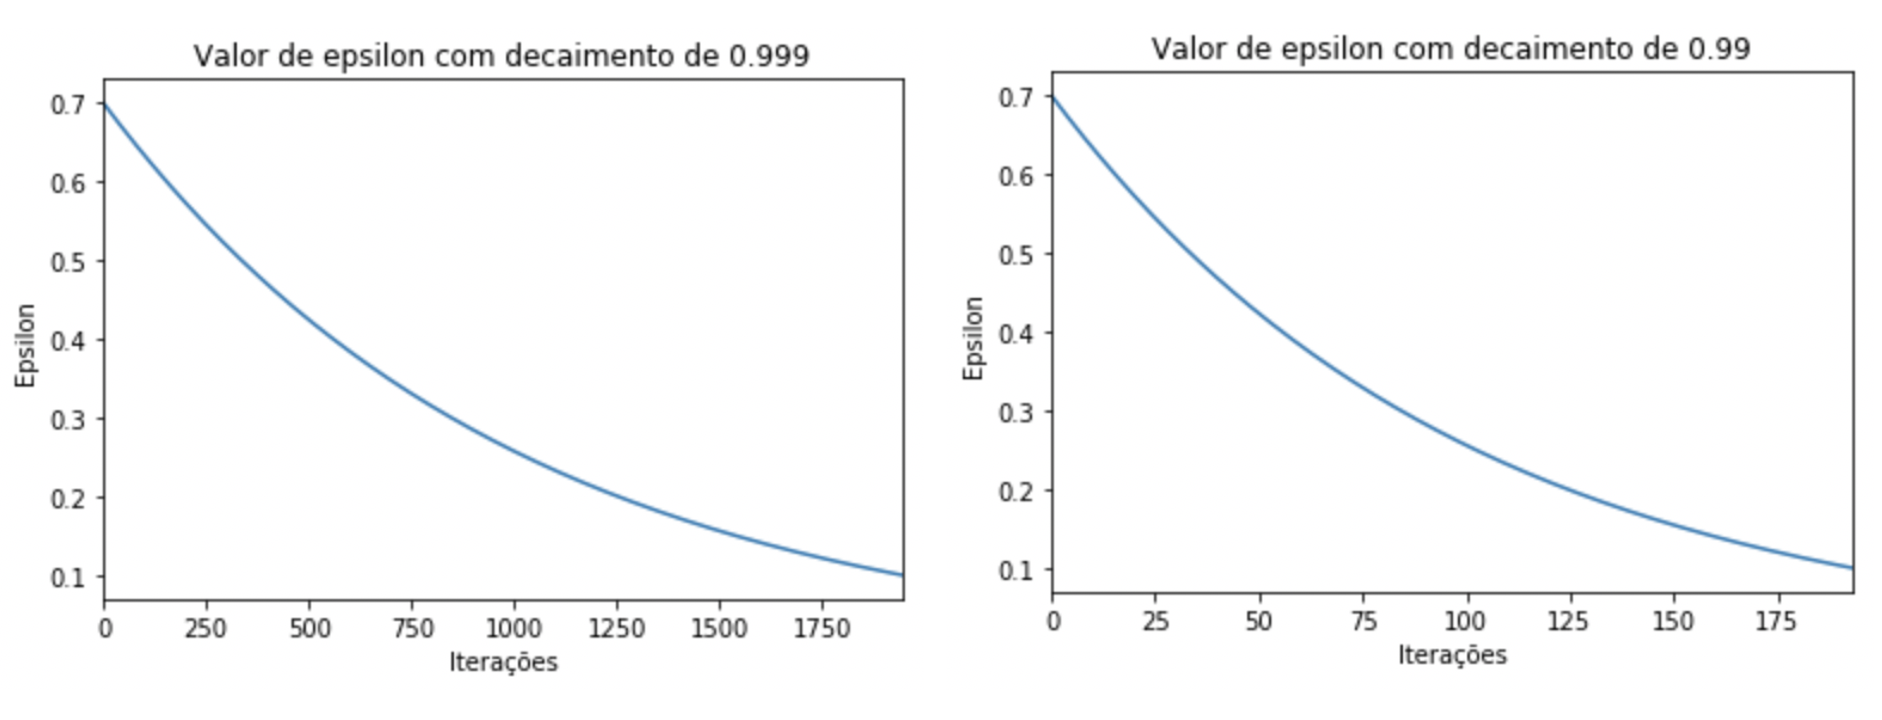
\includegraphics[width=\textwidth]{figuras/epsilon.png}
	\end{center}
\end{frame}

\begin{frame}{Algoritmo Q-Learning}
	
\begin{algorithmic} 
	\STATE \emph{\textbf{function} Q-Learning(env, $\alpha$, $\gamma$, $\epsilon$, $\epsilon_{min}$, $\epsilon_{dec}$, episódios)}
	\STATE inicializar os valores de $Q(s, a)$ arbitrariamente
	\FOR {todos os episódios}
	\STATE inicializar $s$ a partir de $env$
	\REPEAT
	\STATE $a \leftarrow escolha(s, \epsilon)$
	\STATE $s', r \leftarrow$ executar a ação $a$ no $env$
	\STATE $Q(s,a) \leftarrow Q(s,a) + \alpha [r +\gamma \max_{A'}{Q(s', A')} - Q(s,a)]$
	\STATE$s  \leftarrow s'$
	\UNTIL {$s$ ser um estado final}
	\STATE \textbf{if} $\epsilon > \epsilon_{min}$ \textbf{then} $\epsilon \leftarrow \epsilon \times \epsilon_{dec}$
	\ENDFOR
	\STATE \textbf{return} Q
\end{algorithmic}	
\end{frame}

\begin{frame}{Atividade de implementação}
	
	\begin{alertblock}{Implementando o algoritmo Q-Learning}
		O objetivo desta atividade é implementar uma versão do algoritmo Q-Learning
	\end{alertblock}
	
	\begin{block}{Atividades}
		Siga o roteiro descrito em https://insper.github.io/rl/classes/05\_q\_learning/ \href{https://insper.github.io/rl/classes/05_q_learning/}
		{\beamergotobutton{Link}}
	\end{block}
	
\end{frame}

\begin{frame}{Atividade de implementação}
		
	\begin{alertblock}{Hiperparâmetros e seleção das ações}
		O objetivo desta atividade é compreender o funcionamento e impacto dos hiperparâmetros de $\alpha$, $\gamma$ e dos conceitos de \textit{exploration} e \textit{exploitation}.
	\end{alertblock}
	
	\begin{block}{Atividades}
		Siga o roteiro descrito em https://insper.github.io/rl/classes/05\_x\_hyperparameters/ \href{https://insper.github.io/rl/classes/05_x_hyperparameters/}
		{\beamergotobutton{Link}}
	\end{block}

\end{frame}

\begin{frame}{Material de \textbf{consulta}}
	\begin{itemize}
		%\item Tom Mitchell. Machine Learning. McGraw-Hill, 1997.
		\item Richard S. Sutton and Andrew G. Barto. 2018. Reinforcement Learning: An Introduction. A Bradford Book, Cambridge, MA, USA. \textbf{Capítulo 6.5}
		\item Watkins, C.J.C.H., Dayan, P. Q-Learning. Machine Learning 8, 279–292 (1992). \href{https://doi.org/10.1007/BF00992698}{\beamergotobutton{Link}}
		%\item Projeto Gymnasium \href{https://gymnasium.farama.org/}{\beamergotobutton{Link}}
		%\item Projeto PettingZoo \href{https://pettingzoo.farama.org/}{\beamergotobutton{Link}}
		%\item https://deepmind.com/research/case-studies/alphago-the-story-so-far
		\item Aurélien Géron. Hands-On Machine Learning with Scikit-Learn, Keras, and TensorFlow, 2nd Edition, 2019. 
	\end{itemize}
\end{frame}

\end{document}

